%% LyX 2.2.2 created this file.  For more info, see http://www.lyx.org/.
%% Do not edit unless you really know what you are doing.
\documentclass[english,conference,onecolumn]{IEEEtran}
\usepackage[T1]{fontenc}
\usepackage[latin9]{inputenc}
\usepackage{geometry}
\geometry{verbose,tmargin=2cm,bmargin=2cm,lmargin=2cm,rmargin=2cm}
\usepackage{amsmath}
\usepackage{graphicx}

\makeatletter

%%%%%%%%%%%%%%%%%%%%%%%%%%%%%% LyX specific LaTeX commands.
%% Because html converters don't know tabularnewline
\providecommand{\tabularnewline}{\\}

%%%%%%%%%%%%%%%%%%%%%%%%%%%%%% User specified LaTeX commands.
\usepackage{color}
\usepackage{url}
\usepackage[pdfpagemode=None,pdfstartview=FitH,pdfview=FitH,colorlinks=true,pdftitle=The AV1 Constrained Directional Enhancement Filter,pdfauthor=Jean-Marc Valin]{hyperref}

\makeatother

\usepackage{babel}
\begin{document}

\title{The AV1 Constrained Directional Enhancement Filter}

\author{Jean-Marc Valin and Steinar Midtskogen}
\maketitle
\begin{abstract}
This paper presents the constrained directional enhancement filter
designed for the AV1 royalty-free video codec. The filter is based
on a non-linear conditional replacement filter and is designed for
vectorization efficiency. It takes into account the direction of edges
and patterns being filtered. The filter works by identifying the direction
of each block and then adaptively filtering along the identified direction.
In a second pass, the blocks are also filtered with a constrained
low-pass filter. The proposed deringing filter is shown to improve
the quality of the Alliance for Open Media (AOM) AV1 video codec.
\end{abstract}


\section{Introduction}

The main goal of deringing is to filter out ringing artifacts while
retaining all the details of the image. In HEVC, this is achieved
by the Sample Adaptive Offset~(SAO)~\cite{HEVC-SAO} algorithm that
defines signal offsets for different classes of pixels. Unlike SAO,
the approach we take in AV1 is that of a non-linear spatial filter.
From the very beginning, the design of the filter was constrained
to be easily vectorizable (i.e. implementable with SIMD operations),
which was not the case for other non-linear filters like the median
filter~\cite{Median} and the bilateral filter~\cite{Bilateral}. 

The design of the deringing filter originates from the following observations.
The amount of ringing in a coded image tends to be roughly proportional
to the quantization step size. The amount of detail is a property
of the input image, but the smallest detail actually retained in the
quantized image tends to also be proportional to the quantization
step size. For a given quantization step size, the amplitude of the
ringing is generally less than the amplitude of the details.

This paper describes the constrained directional enhancement filter
(CDEF), a deringing filter that takes into account the direction of
edges and patterns being filtered. CDEF works by identifying the direction
of each block and then adaptively filtering along the identified direction.
In a second pass, the blocks are also filtered with a constrained
low-pass filter, and with more conservative strength to avoid blurring
edges. The deringing filter also vectorizes well, requiring no per-pixel
scalar operation. An high-level interactive demonstration of the algorithm
is available at~\cite{deringing-demo}.

\section{Direction Search}

The proposed deringing filter is based on the direction of edges,
so we will start by describing the direction search. For this, the
image is first divided into blocks of $8\times8$. The block size
is chosen to be fine enough to adequately handle non-straight edges,
while being large enough to reliably estimate directions when applied
to a quantized image. Having a constant direction over an $8\times8$
region also makes vectorization of the filter easier.

For each block we want to determine the direction that best matches
the pattern in the block. This is done by minimizing the sum of squared
differences (SSD) between the quantized block and a perfectly directional
block. A perfectly directional block is a block for which each line
along a certain direction has a constant value. For each direction,
we assign a line number $k$ to each pixel, as shown in Fig.~\ref{fig:Lines-for-direction}. 

\begin{figure}
\centering{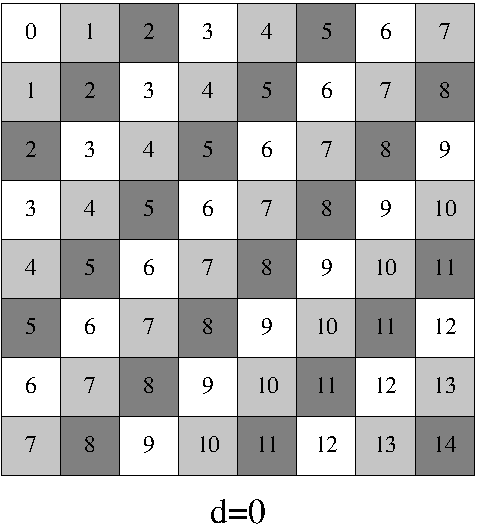
\includegraphics[width=0.2\textwidth]{dlines0}\hspace{1.5em}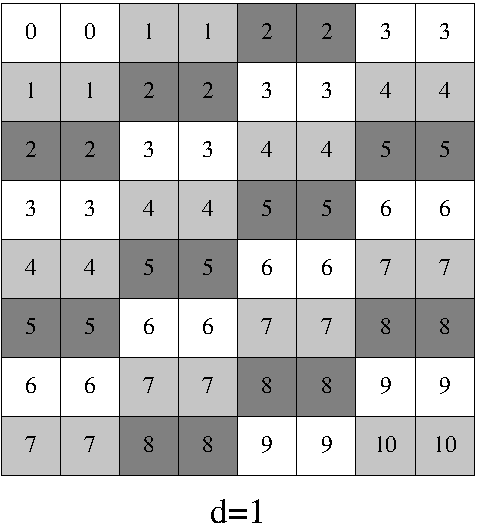
\includegraphics[width=0.2\textwidth]{dlines1}\hspace{1.5em}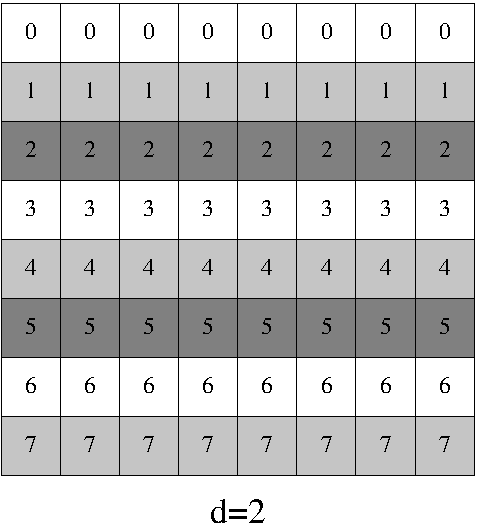
\includegraphics[width=0.2\textwidth]{dlines2}\hspace{1.5em}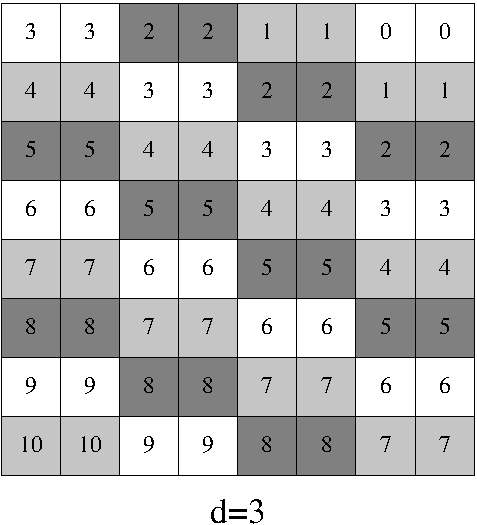
\includegraphics[width=0.2\textwidth]{dlines3}}

\vspace{1.5em}

\centering{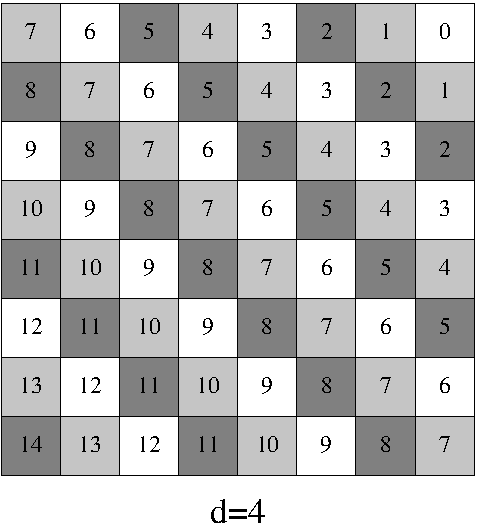
\includegraphics[width=0.2\textwidth]{dlines4}\hspace{1.5em}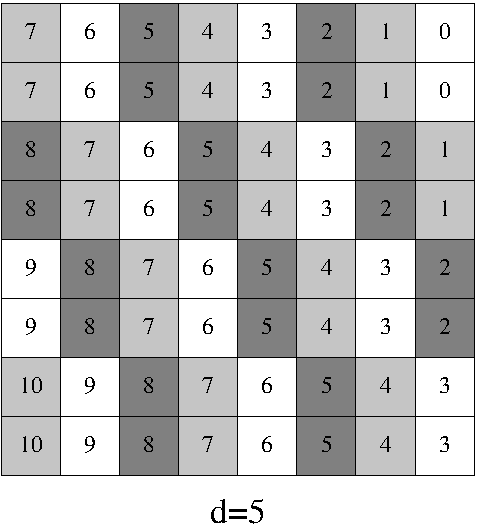
\includegraphics[width=0.2\textwidth]{dlines5}\hspace{1.5em}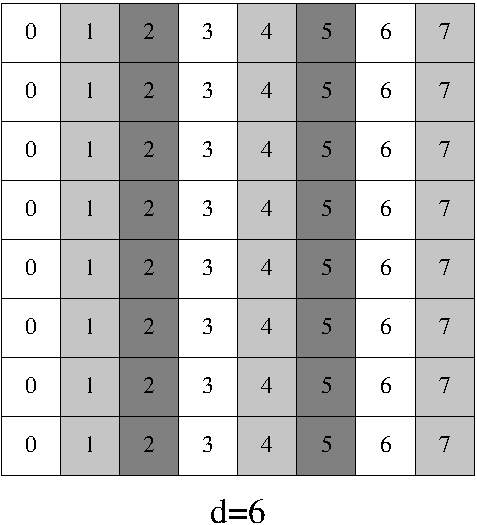
\includegraphics[width=0.2\textwidth]{dlines6}\hspace{1.5em}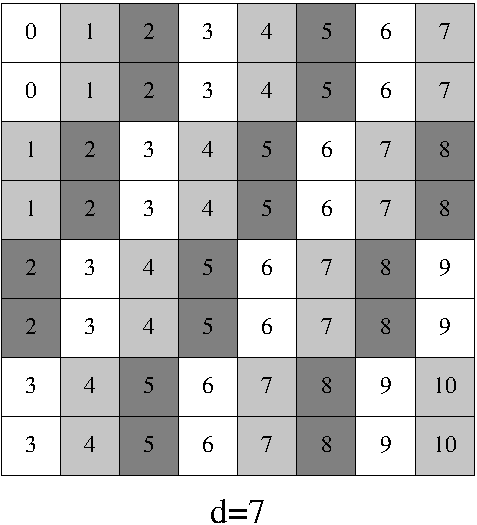
\includegraphics[width=0.2\textwidth]{dlines7}}\caption{Line number $k$ for pixels following direction $d=0:7$ in an $8\times8$
block.\label{fig:Lines-for-direction}}
\end{figure}

For each direction $d$, the pixel average for line $k$ is determined
by:
\begin{equation}
\mu_{d,k}=\frac{1}{N_{d,k}}\sum_{p\in P_{d,k}}x_{p}\ ,\label{eq:pixel-average}
\end{equation}
where $x_{p}$ is the value of pixel $p$, $P_{d,k}$ is the set of
pixels in line $k$ following direction $d$ and $N_{d,k}$ is the
cardinality of $P_{d,k}$ (for example, in Fig.~\ref{fig:Lines-for-direction},
$N_{1,0}=2$ and $N_{1,4}=8$). The SSD is then defined as:
\begin{equation}
\sigma_{d}^{2}=\sum_{k\in\mathrm{block},d}\left[\sum_{p\in P_{d,k}}\left(x_{p}-\mu_{d,k}\right)^{2}\right]\ .\label{eq:direction-variance0}
\end{equation}

Expanding (\ref{eq:direction-variance0}) and then substituting (\ref{eq:pixel-average})
into it, we get
\begin{align}
\sigma_{d}^{2}= & \sum_{k\in\mathrm{block},d}\left[\sum_{p\in P_{d,k}}x_{p}^{2}-2\sum_{p\in P_{d,k}}x_{p}\mu_{d,k}+\sum_{p\in P_{d,k}}\mu_{d,k}^{2}\right]\nonumber \\
= & \sum_{k\in\mathrm{block},d}\left[\sum_{p\in P_{d,k}}x_{p}^{2}-2\mu_{d,k}\sum_{p\in P_{d,k}}x_{p}+N_{d,k}\mu_{d,k}^{2}\right]\nonumber \\
= & \sum_{k\in\mathrm{block},d}\left[\sum_{p\in P_{d,k}}x_{p}^{2}-\frac{1}{N_{d,k}}\left(\sum_{p\in P_{d,k}}x_{p}\right)^{2}\right]\nonumber \\
= & \sum_{p\in\mathrm{block}}x_{p}^{2}-\sum_{k\in\mathrm{block},d}\frac{1}{N_{d,k}}\left(\sum_{p\in P_{d,k}}x_{p}\right)^{2}\ .\label{eq:direction-variance1}
\end{align}
 Note that the simplifications leading to (\ref{eq:direction-variance1})
are the same as to those allowing a variance to be computed as $\sigma_{x}^{2}=\sum x^{2}-\left(\sum x\right)^{2}/N$.
Considering that the first term of (\ref{eq:direction-variance1})
is constant with respect to $d$, we simply find the optimal direction
$d_{opt}$ by maximizing the second term:
\begin{equation}
d_{opt}=\max_{d}s_{d}\,,\label{eq:direction-variance2}
\end{equation}
where 
\begin{equation}
s_{d}=\sum_{k\in\mathrm{block},d}\frac{1}{N_{d,k}}\left(\sum_{p\in P_{d,k}}x_{p}\right)^{2}\ .\label{eq:direction-variance3}
\end{equation}

We can avoid the division in (\ref{eq:direction-variance3}) by multiplying
$s_{d}$ by 840, the least common multiple of the possible $N_{d,k}$
values ($1\le N_{d,k}\le8$). When using 8\nobreakdash-bit pixel
data (for higher bit depths, we downscale to 8~bits), and centering
the values such that $-128\le x_{p}\le127$, then $840s_{d}$ and
all calculations leading to that value fit in a 32\nobreakdash-bit
signed integer.

Fig. \ref{fig:Example-of-direction} shows an example of a direction
search for an $8\times8$ block containing a line. 

\begin{figure}
\centering{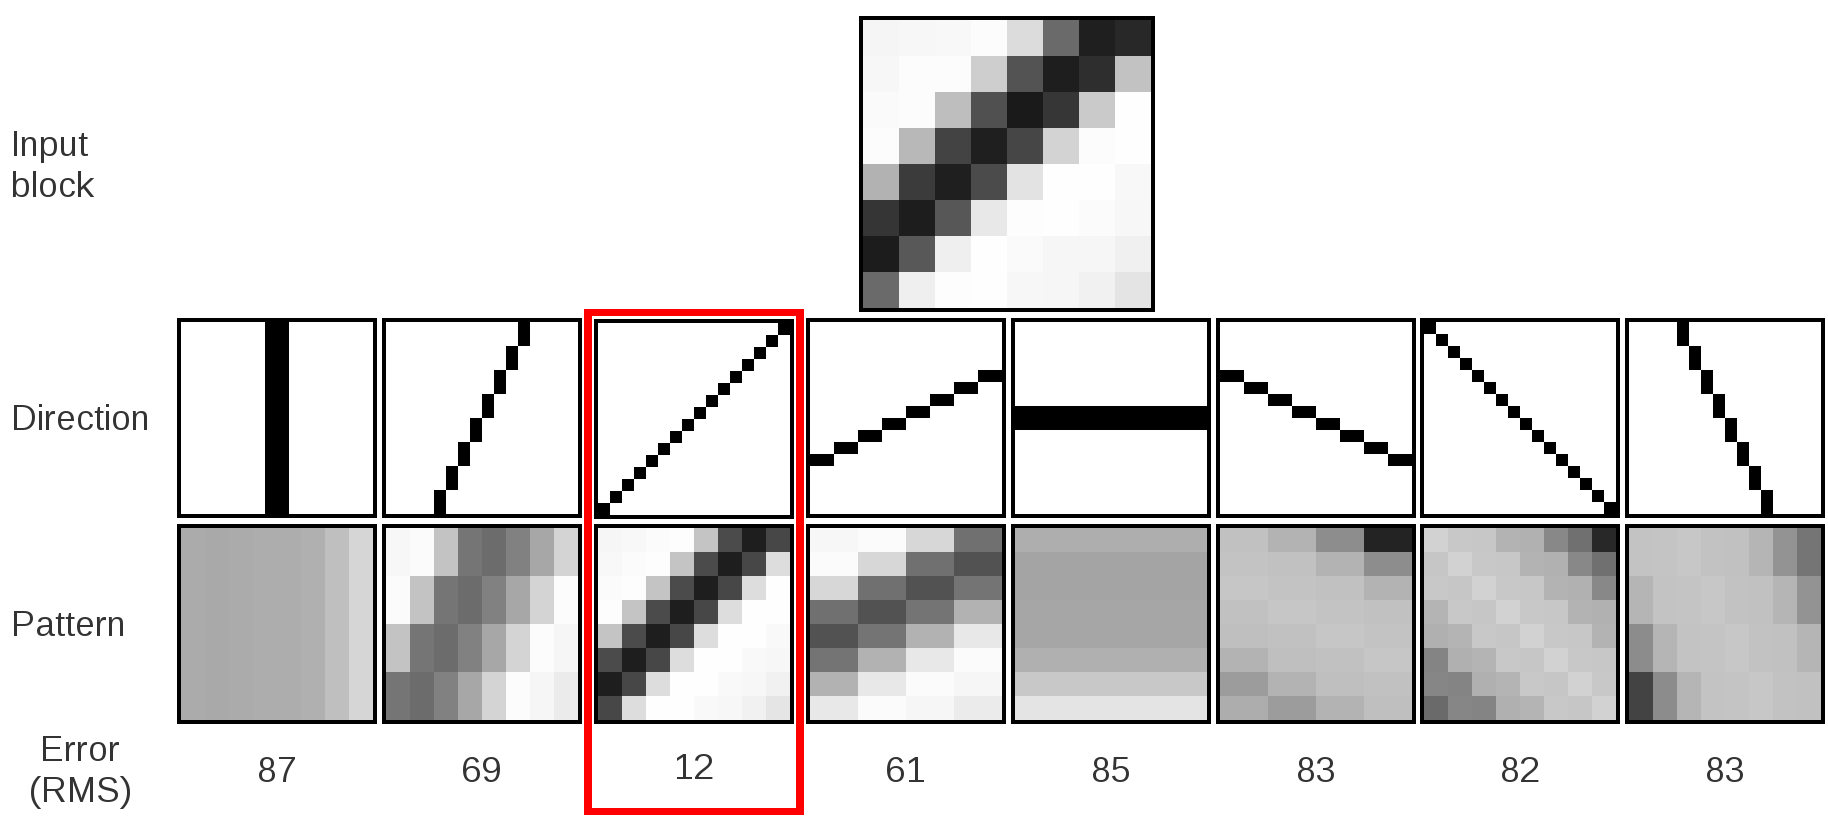
\includegraphics[width=0.6\columnwidth]{direction}}\caption{Example of direction search for an $8\times8$ block. The patterns
shown are based on the $\mu_{d,k}$ values. In this case, the 45-degree
direction is the one that minimizes $\sigma_{d}^{2}$, so it would
be selected by the search. Note that the error values $\sigma_{d}$
shown are never computed in practice (only $s_{d}$ is). \label{fig:Example-of-direction}}

\end{figure}


\section{Conditional Replacement Filter}

The conditional replacement filter is designed to remove noise without
blurring sharp edges. A low-pass finite impulse response (FIR) filter
with $\left(2M+1\right)$ taps in one dimension can be expressed as
\begin{equation}
y\left(n\right)=\frac{1}{W}\sum_{k=-M}^{k=M}w_{k}x\left(n+k\right)\ ,\label{eq:linear-filter}
\end{equation}
where $W=\sum_{k=-M}^{M}w_{k}$. Although it removes noise from a
signal, it also blurs any details and sharp edges, which is undesirable.
Bilateral filters avoid the blurring effect by making each weights
$w_{k}$ dependent on the difference signal $x\left(n+k\right)-x\left(n\right)$,
typically using a Gaussian function. One disadvantage of this approach
is that it requires keeping track of the sum of the weights for each
sample $n$ being filtered. It also results in having a different
$\frac{1}{W}$ normalization factor for each pixel, making vectorization
harder. 

Rather than change the $w_{k}$ values, the conditional replacement
filter changes the signal $x\left(n+k\right)$ used in the filter.
When filtering sample $n$, any of the $x\left(n+k\right)$ tap inputs
that differs from $x\left(n\right)$ by more than a threshold $T$,
is replaced by $x\left(n\right)$ in the calculation:
\begin{equation}
y\left(n\right)=\frac{1}{W}\sum_{k=-M}^{k=M}w_{k}R\left(x\left(n\right),x\left(n+k\right),T\right)\ ,\label{eq:crf-definition}
\end{equation}
with
\begin{equation}
R\left(x_{0},x_{k},T\right)=\begin{cases}
x_{k} & ,\left|x_{k}-x_{0}\right|<T\\
x_{0} & ,\mathrm{otherwise}
\end{cases}\ .\label{eq:crf-replacement}
\end{equation}
 The filter computation is illustrated in Fig.~\ref{fig:Conditional-filter-computation}
and an example is shown in Fig.~\ref{fig:Conditional-filter-example}.

\begin{figure}
\centering{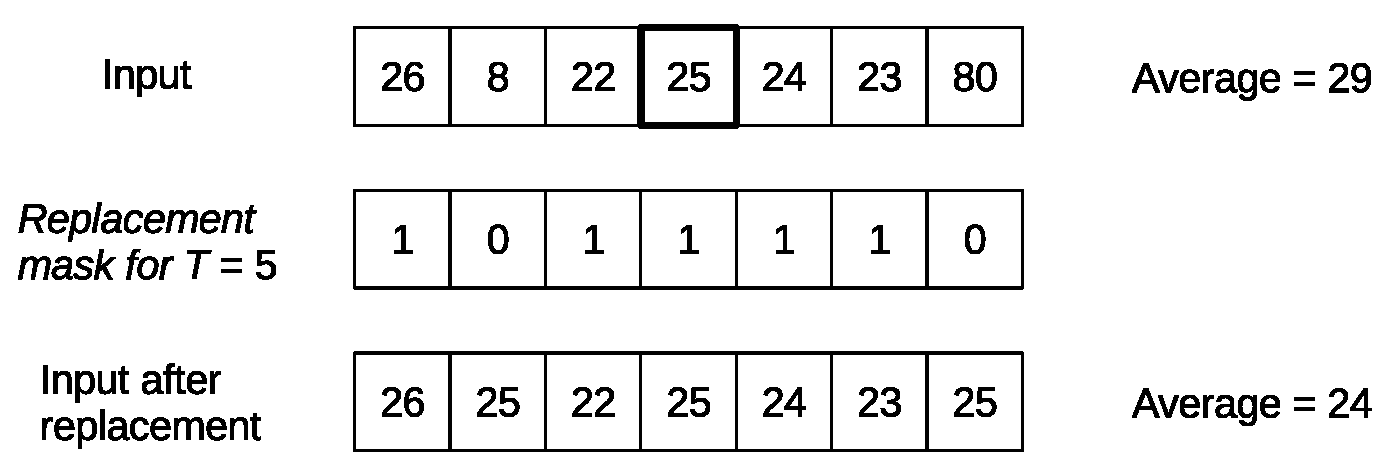
\includegraphics[width=0.5\textwidth]{crf_def}}

\caption{Conditional replacement filter computation\label{fig:Conditional-filter-computation}}

\end{figure}

\begin{figure}
\centering{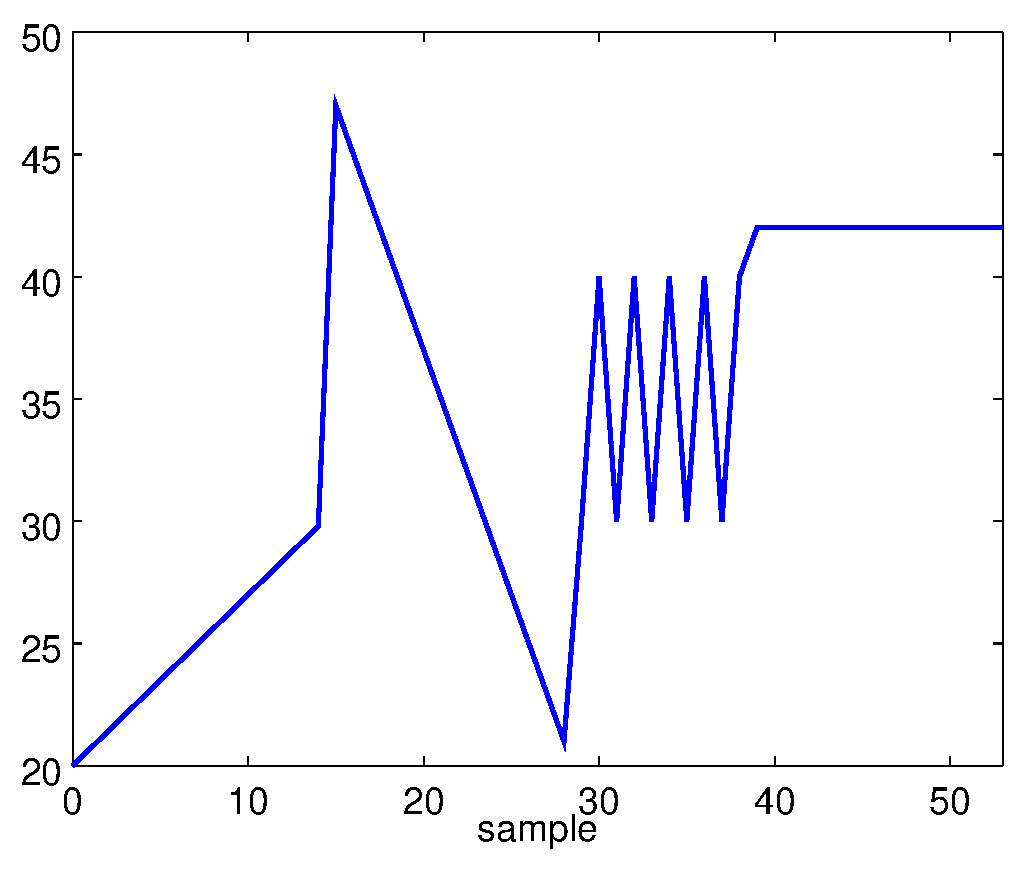
\includegraphics[width=0.3\columnwidth]{crf_orig}\hspace{2mm}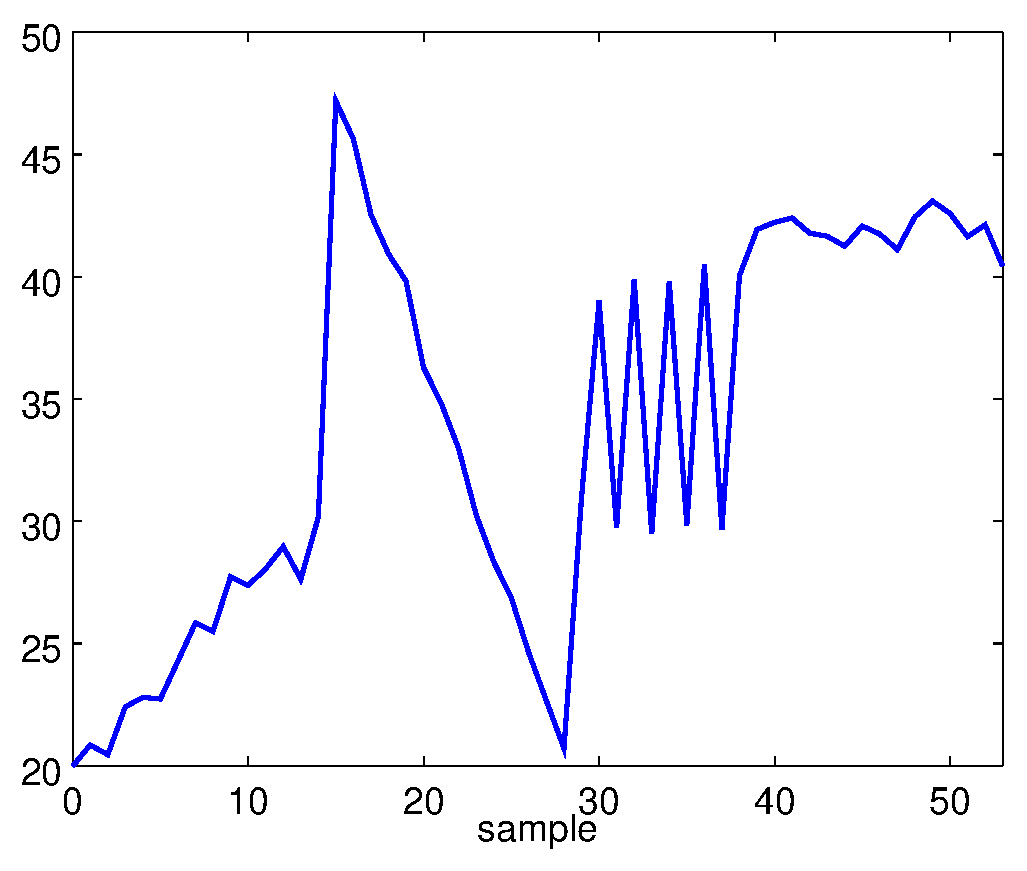
\includegraphics[width=0.3\columnwidth]{crf_noisy}

\vspace{2mm}

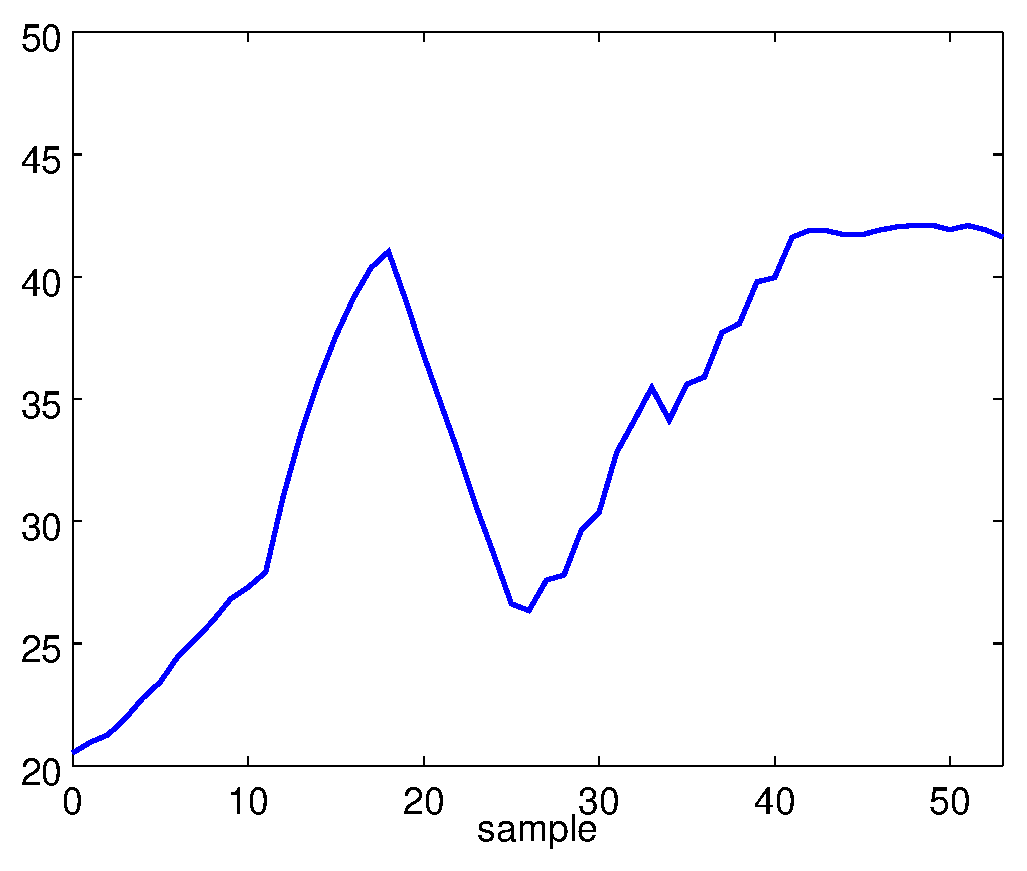
\includegraphics[width=0.3\columnwidth]{crf_linear}\hspace{2mm}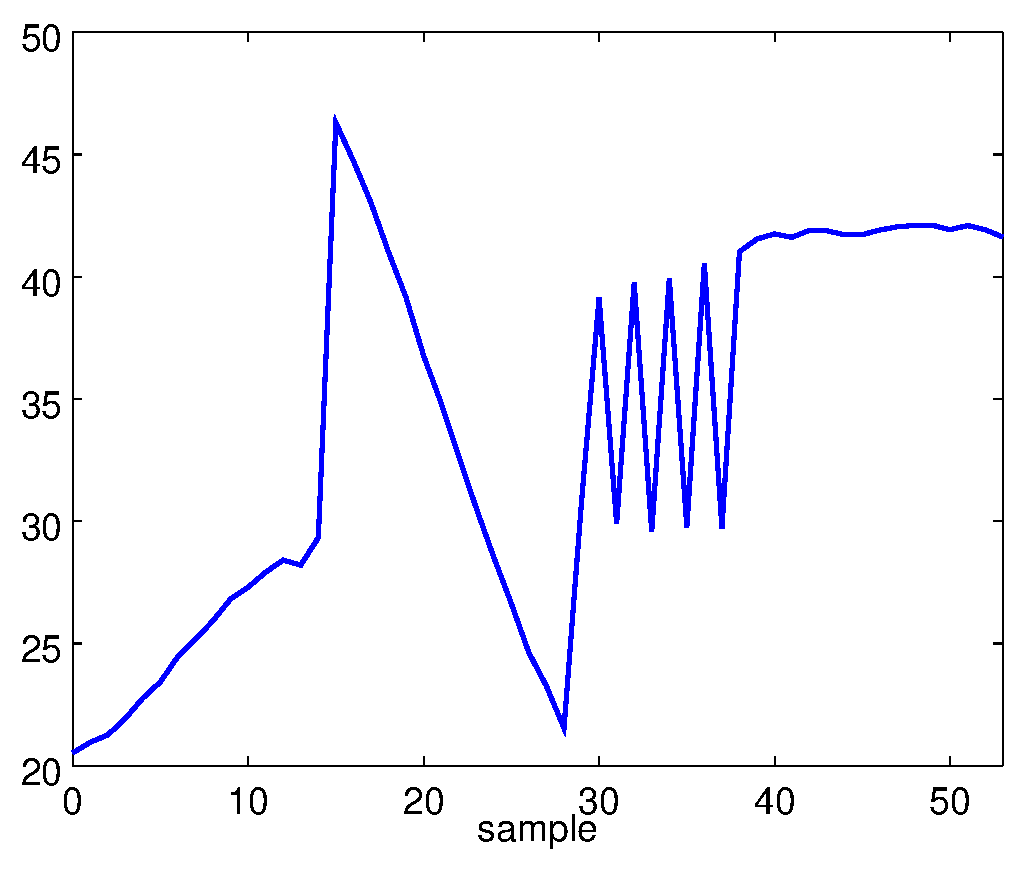
\includegraphics[width=0.3\columnwidth]{crf_out}}

\caption{Conditional replacement filter example. Up-left: original signal,
up-right: noisy signal, bottom-left: filtered with 7-tap linear filter,
bottom-right: filtered with 7-tap conditional replacement filter.
\label{fig:Conditional-filter-example}}
\end{figure}

Through algebraic simplifications, we can express the filter (\ref{eq:crf-definition})
in terms of the differences $x\left(n+k\right)-x\left(n\right)$,
which yields
\begin{equation}
y\left(n\right)=x\left(n\right)+\frac{1}{W}\sum_{k=-M,k\neq0}^{k=M}w_{k}f\left(x\left(n+k\right)-x\left(n\right),T\right)\ ,\label{eq:conditional-replacement-diff}
\end{equation}
with the threshold function 
\begin{equation}
f\left(d,T\right)=\left\{ \begin{array}{ll}
d & ,\left|d\right|<T\\
0 & ,\mathrm{otherwise}
\end{array}\right.\ .\label{eq:threshold-function}
\end{equation}
The advantage of this formulation is that the normalization by $\frac{1}{W}$
can be approximated without causing any bias (DC offset), even when
$W$ is not a power of two. Also, because $W$ does not depend on
the number of pixels being replaced, the normalization is easy to
vectorize over a row (or column) of pixels. 

The directional filter for pixel $\left(i,j\right)$ is defined as
the 7-tap conditional replacement filter
\begin{multline}
y\left(i,j\right)=x\left(i,j\right)+\frac{1}{W}\sum_{k=-3,\,k\neq0}^{3}w_{k}f\left[x\left(i,j\right)-\right.\\
\left.x\left(i+\left\lfloor kd_{y}\right\rfloor ,j+\left\lfloor kd_{x}\right\rfloor \right),T_{d}\right]\label{eq:directional_filter}
\end{multline}
where $d_{x}$ and $d_{y}$ define the direction, $W$ is a constant
normalizing factor, $T_{d}$ is the filtering threshold for the block.
The direction parameters are shown in Table~\ref{tab:Direction-parameters}.
The weights $w_{k}$ can be chosen so that $W$ is a power of two.
For example, Daala currently uses $\mathbf{w}=\left[\begin{array}{ccccccc}
1 & 2 & 3 & \left(4\right) & 3 & 2 & 1\end{array}\right]$ (where the middle value of 4 is implicit) with $W=16$. Since the
direction is constant over $8\times8$ blocks, all operations in this
filter are directly vectorizable over the blocks. 

\begin{table}
\caption{Direction parameters\label{tab:Direction-parameters}}
\centering{%
\begin{tabular}{ccrr}
\hline 
Index & Direction & $d_{x}$ & $d_{y}$\tabularnewline
\hline 
0 & \rotatebox[origin=c]{45}{$\leftrightarrow$} & $1$ & $-1$\tabularnewline
1 & \rotatebox[origin=c]{22.5}{$\leftrightarrow$} & $1$ & $-\frac{1}{2}$\tabularnewline
2 & \rotatebox[origin=c]{0}{$\leftrightarrow$} & $1$ & $0$\tabularnewline
3 & \rotatebox[origin=c]{-22.5}{$\leftrightarrow$} & $1$ & $\frac{1}{2}$\tabularnewline
4 & \rotatebox[origin=c]{-45}{$\leftrightarrow$} & $1$ & $1$\tabularnewline
5 & \rotatebox[origin=c]{-65.5}{$\leftrightarrow$} & $\frac{1}{2}$ & $1$\tabularnewline
6 & \rotatebox[origin=c]{-90}{$\leftrightarrow$} & $0$ & $1$\tabularnewline
7 & \rotatebox[origin=c]{-112.5}{$\leftrightarrow$} & $-\frac{1}{2}$ & $1$\tabularnewline
\hline 
\end{tabular}}

\end{table}

\begin{figure}
\centering{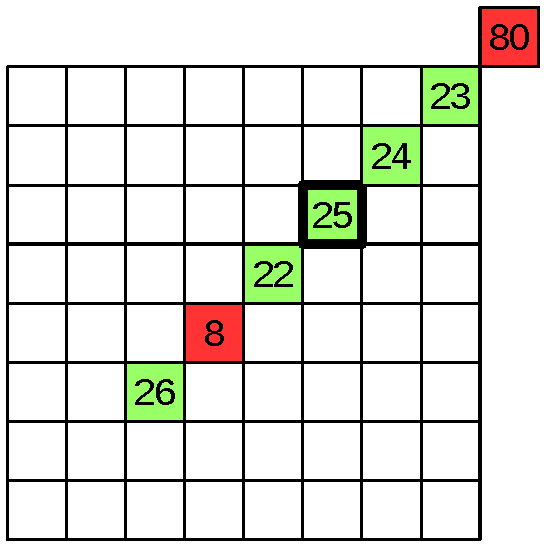
\includegraphics[width=0.3\columnwidth]{crf_direction}}

\caption{Filtering along the direction (left)\label{fig:Filtering-along-across}. }
\end{figure}


\subsection{Setting the Threshold}

The threshold $T_{d}$ must be set high enough to smooth out ringing
artifacts, but low enough to avoid blurring important details in the
image. Although the ringing is \emph{roughly} proportional to the
quantization step size $Q$, as the quantizer increases the error
grows slightly less than linearly because the unquantized coefficients
become very small compared to $Q$. As a starting point for determining
the thresholds, we can use a power model of the form
\begin{equation}
T_{0}=\alpha_{1}Q^{\beta}\ell\ ,\label{eq:setting-Td}
\end{equation}
with $\beta=0.6$, and where $\alpha_{1}$ depends on the input scaling.
The deringing \emph{level} $\ell$ is a threshold adjustment coded
for each superblock ($64\times64$). The level can take one of 4 values:
\begin{equation}
\ell\in\left\{ 0,\,11/16,\,1,\,22/16\right\} \ ,
\end{equation}
where $\ell=0$ disables the deringing filter for the current superblock. 

Another factor that affects the optimal filtering threshold is the
presence of strong directional edges/patterns. These can be estimated
from the $s_{d}$ parameters computed in Eq.~(\ref{eq:direction-variance3})
as
\begin{equation}
\delta=s_{d_{opt}}-s_{d_{ortho}}\ ,\label{eq:variande-delta}
\end{equation}
where $d_{ortho}=d_{opt}+4\ \left(\mathrm{mod}\,8\right)$. We compute
the direction filtering threshold for each block as 
\begin{equation}
T_{d}=T_{0}\cdot\max\left(\tfrac{1}{2},\min\left(3,\alpha_{2}\delta^{1/6}\right)\right)\ ,\label{eq:threshold-pow}
\end{equation}
where $\alpha_{2}$ also depends on the input scaling. 

As a special case, when the pixels corresponding to the $8\times8$
block being filtered are all skipped, then $T_{d}=0$, so no deringing
is performed. Aside from frame header information, the level $\ell$
is the only information coded in the bitstream for the directional
filter. More specifically, neither $\delta$ nor the direction $d$
are coded, since they are computed by the decoder. The level is not
currently entropy coded, but that is likely to change in the future. 

\section{Constrained Low-Pass Filter}

The 7-tap directional filter is sometimes not enough to eliminate
all ringing, so we use an additional filtering step that operates
across the direction lines used in the first filter. Considering that
the input of the second filter has considerably less ringing than
the input of the first filter, and the risk of blurring edges, the
strength of the second filter needs to be smaller.

The constrained low-pass filter (CLPF) used as the second filter is
a variant of the conditional replacement filter. It is applied to
the luma and chroma planes after the first directional filter. The
filter block (FB) size and filter strength are signalled once per
frame. Tile groups must signal the same values for FB size and strength.
A value of 0 for the FB size means that FB signalling is disabled
(see below) and 1, 2 and 3 mean that the FB size is 32x32, 64x64 and
128x128 respectively. The filter strength can be 1, 2 or 4 (signalled
as \textquotedblleft 3\textquotedblright ) for 8 bit content. For
higher bit content the strength is scaled accordingly, so for 10 bit
content the strengths are 4, 8 or 16. Skip blocks (blocks without
residuals) are not filtered if the FB size is 32x32 or 64x64.

The luma and chroma planes are filtered independently, each with its
own strength, but only luma can have FB signalling. The filter can
be enabled/disabled at FB level in the luma plane by sending one bit
for a FB if the following conditions are true:
\begin{enumerate}
\item FB-level signaling is enabled (FB size set to 32x32, 64x64 or 128x128) 
\item The FB size is 128x128 or at least one block within the FB is not
a skip block if the FB size is 32x32 or 64x64
\end{enumerate}
If a 32x32 or 64x64 FB is entirely made up of skip blocks, no bit
is sent for that FB and it\textquoteright s not filtered.For blocks
to be filtered the following operation is performed, where A, B, C,
D, E, F, G, H and the pixel to be filtered X are organized in the
pattern shown in Figure~\ref{fig:clpf_taps}, and $s$ denotes the
filter strength: 

\begin{align*}
X'=X+[ & g\left(A-X,s\right)+3g\left(B-X,s\right)+\\
 & g\left(C-X,s\right)+3g\left(D-X,s\right)+\\
 & g\left(F-X,s\right)+3g\left(E-X,s\right)+\\
 & g\left(H-X,s\right)+3g\left(G-X,s\right)]/16
\end{align*}
where the constraint function is defined as
\[
g\left(d,s\right)=\mathrm{sign}\left(d\right)\max\left(0,\left|d\right|-\max\left(0,\left|d\right|-s+2^{3-B+\log_{2}s}\left|d\right|\right)\right)
\]
where $B$ is the bit depth (8-, 10-, or 12-bit). The constraint restricts
the range gradually down to 0 as the pixel difference $\left|d\right|$
approaches 32 (128, 512) for 8 (10, 12) bit content. The intention
is to reduce the effect of dissimilar neighbouring pixels. Figure~\ref{fig:Constrain-function}
illustrates the effect of the function.

\begin{figure}

\centering{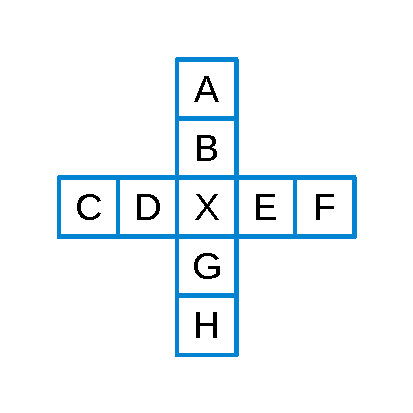
\includegraphics[width=0.3\textwidth]{clpf}}

\caption{Constrained low-pass fitler taps\label{fig:clpf_taps}}

\end{figure}

\begin{figure}
\centering{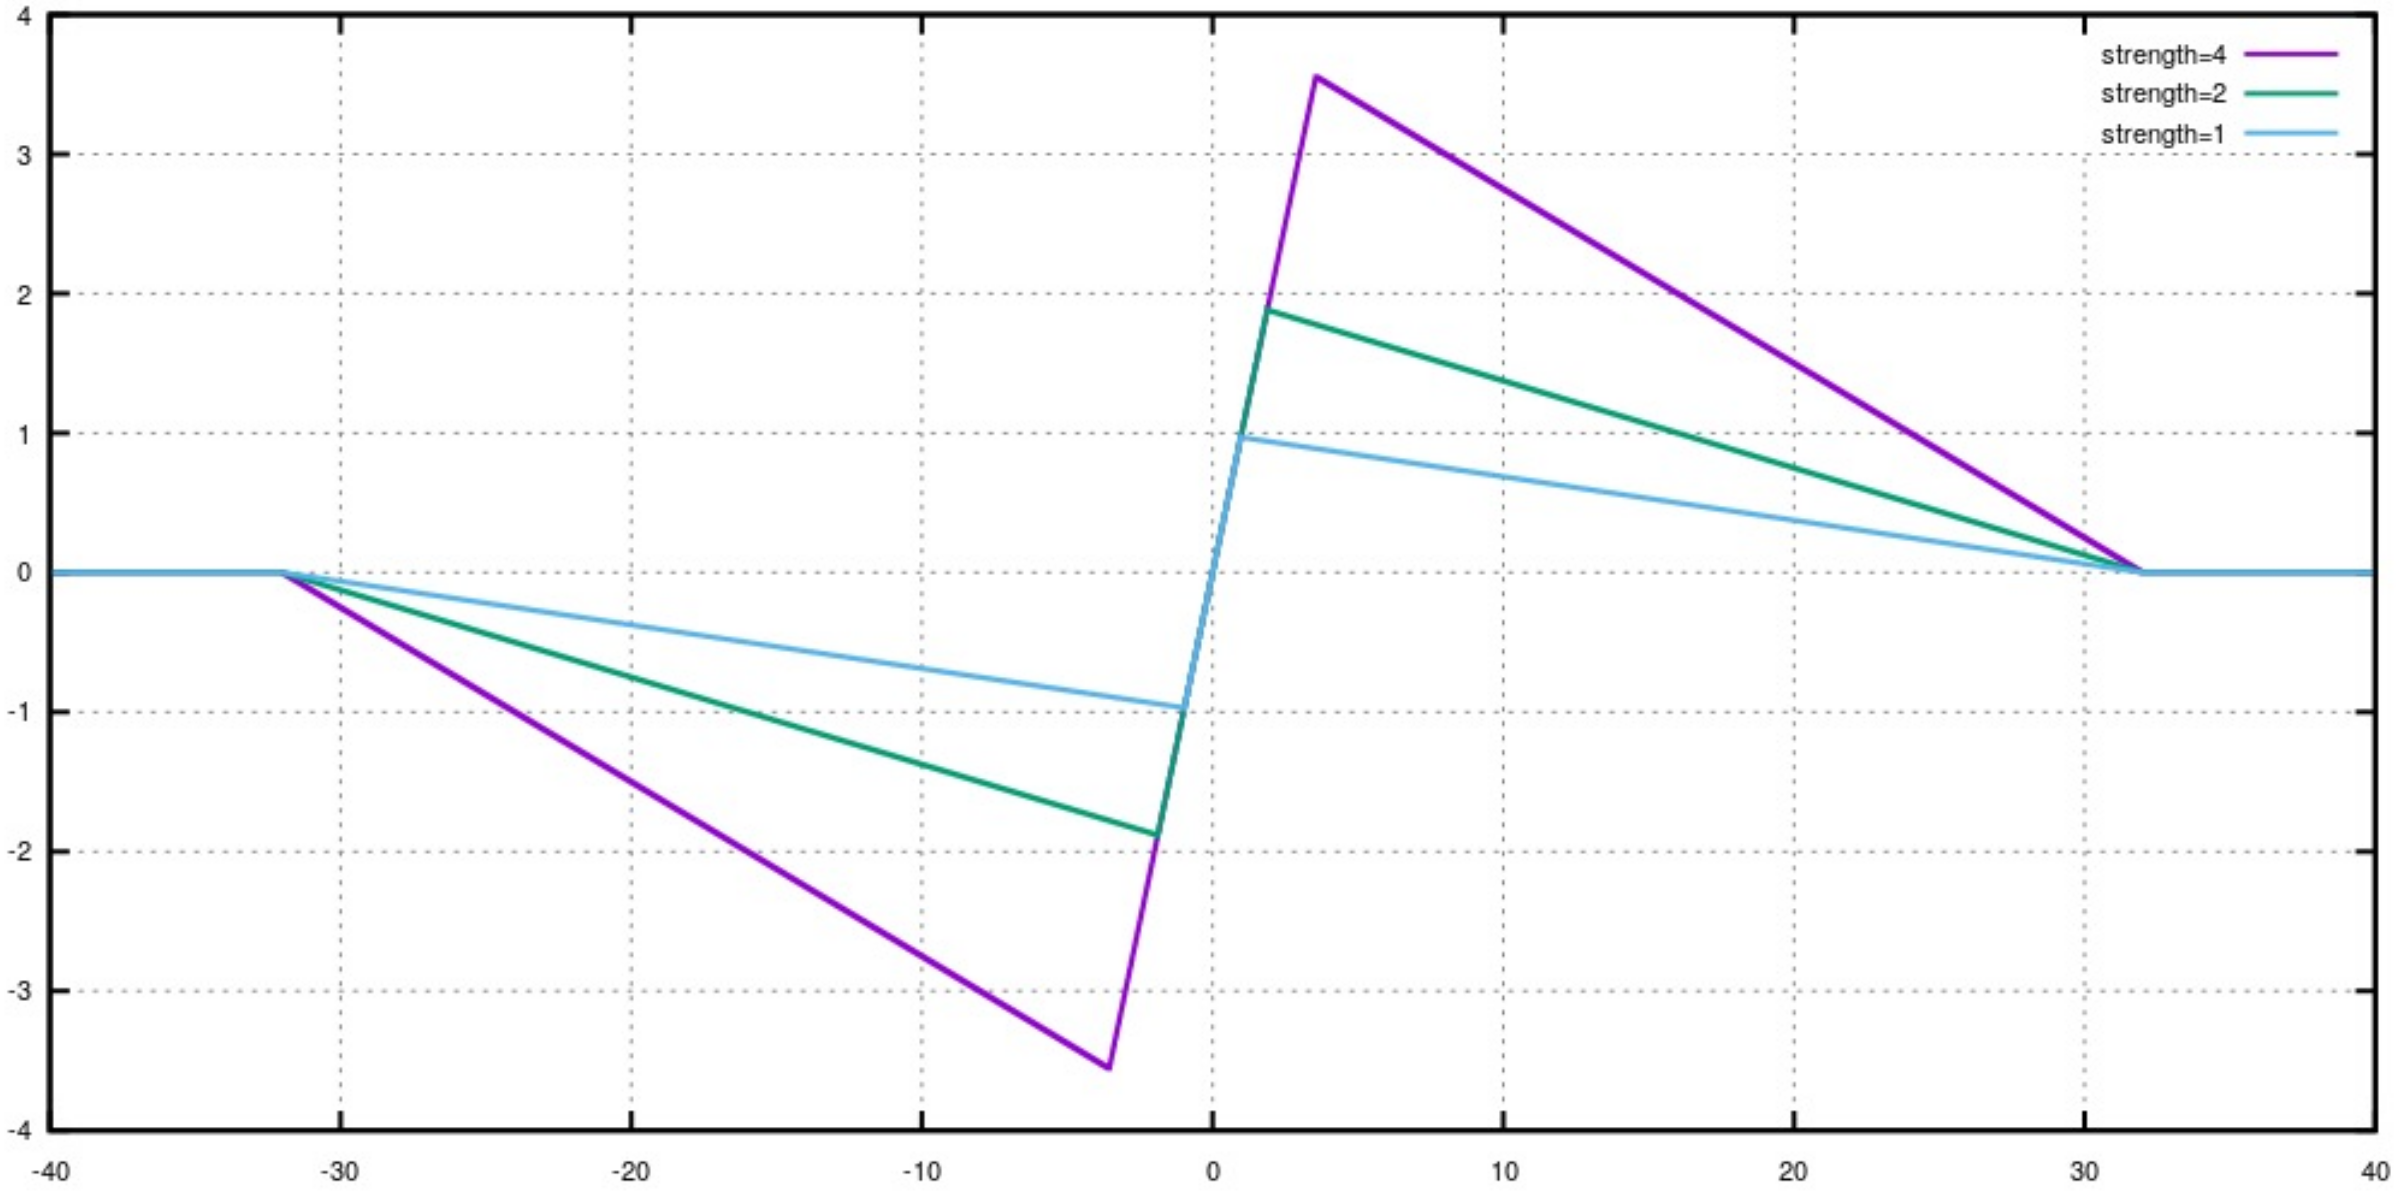
\includegraphics[width=0.7\textwidth]{clpf_func}}

\caption{Constrain function\label{fig:Constrain-function}}
\end{figure}

The filter rounds to the nearest integer. If an input pixel is outside
the frame border, the nearest pixel inside the frame is used. When
FB signalling is enabled, up to four bits are transmitted per superblock
(SB) when the FB size is 32x32, 0 or 1 bit per SB if the FB size is
64x64, and when the FB size is 128x128, there is always 1 bit for
every top left SB of the FB. Note that when the size is 128x128, even
skip blocks within the FB get filtered if the filter is enabled for
the FB.

As a way to reduce the number of buffered lines, we only use the horizontal
taps of CLPF when the direction is 0, 4, 5, 6, or 7.

\section{Superblocks and Signaling}

The filtering is applied one superblock at a time. On inter-predicted
frames, the filter parameters are only coded for superblocks that
are not skipped. Superblocks where no level is coded have CDEF disabled.
Similarly, any skipped block within a superblock has all filtering
disabled, even if it is signaled enabled for the superblock. 

The CDEF process sometimes reads pixels that lie outside of the superblock
being processed. When these pixels belong to another superblock, the
filtering always uses the unfiltered pixel values \textendash{} even
for the second filter (CLPF) \textendash{} so that no dependency is
added between the superblocks. This makes it possible to filter all
superblocks in parallel. When the pixels used for a filter lie outside
of the viewable image, we set $f\left(d,T\right)=0$ in Eq.~(\ref{eq:threshold-function}).

\section{Decoder Process}

For each 8x8 block, the following steps are applied.

\subsection{Direction Search}

The direction search evaluates equation (\ref{eq:direction-variance3})
for each of the 8 directions, with the $\frac{1}{N_{d,k}}$ factor
being replaced by a 10-bit multiply. In total, the search for all
8 directions requires the following arithmetic operations:
\begin{enumerate}
\item The pixel accumulations in equation (\ref{eq:direction-variance3})
are 418 adds of 8-bit signed values, with results that fit in 11 bits.
There's a maximum of 8 values contributing to each sums. (there are
simplifications that can save 128 adds using intermediate sums).
\item The result of 1) is 90 11-bit partial sums. Each is squared (so 90
11-bit multiplies), with the result being 21-bit unsigned values.
Each of these is multiplied by one of eight different 10-bit constants,
with the result guaranteed to fit in 27 bits. Since some lines use
the same constant and are eventually added together, only 34 multiplies
by constants are needed after simplification. 
\item There are another 86 adds from the results of step 2), resulting in
8 29-bit unsigned values. There's a maximum of 15 values contributing
to each of these sums.
\item The resulting values in 3) are compared to find the largest value. 
\end{enumerate}

\subsection{Threshold Computation}

The threshold to use for the block is obtained by approximating equation
(\ref{eq:threshold-pow}) using a lookup table.

\subsection{Directional Filter}

For luma, we use a 7-tap filter along the direction found in the direction
search. For each pixel $X$, the new value $X'$ is computed as
\begin{align*}
X'=X+[ & f\left(A-X,T\right)+2f\left(B-X,T\right)+\\
 & 3f\left(C-X,T\right)+3f\left(D-X,T\right)+\\
 & 2f\left(E-X,T\right)+f\left(F-X,T\right)]/16
\end{align*}
where $f\left(d,T\right)$ is defined in equation (\ref{eq:threshold-function})
and the direction-dependent position of the taps is shown in Fig.~(\ref{fig:Position-of-taps}). 

\begin{figure}
\centering{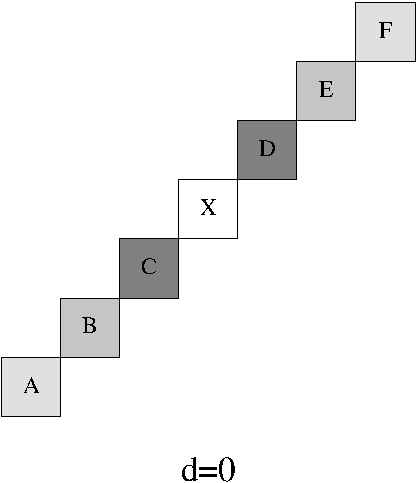
\includegraphics[scale=0.5]{taps0}\hspace{1.5em}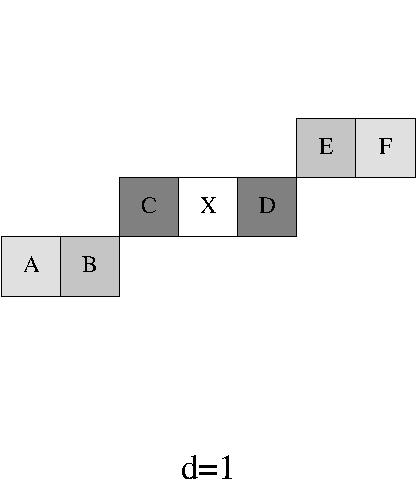
\includegraphics[scale=0.5]{taps1}\hspace{1.5em}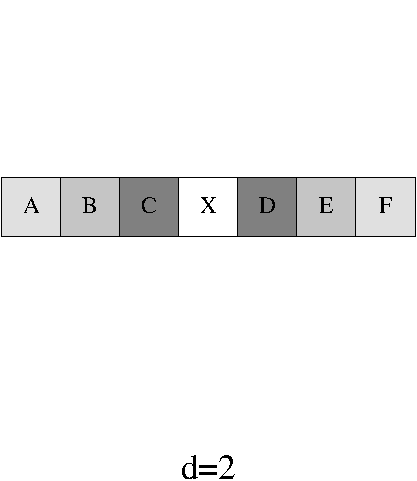
\includegraphics[scale=0.5]{taps2}\hspace{1.5em}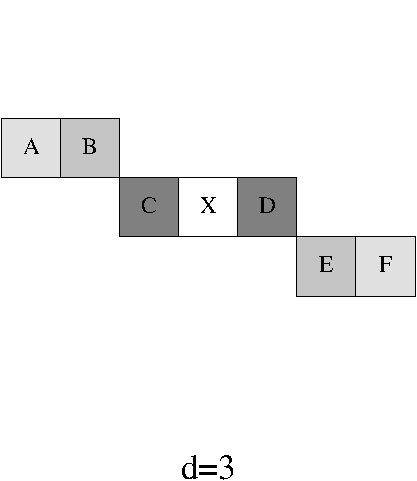
\includegraphics[scale=0.5]{taps3}}

\vspace{2em}

\centering{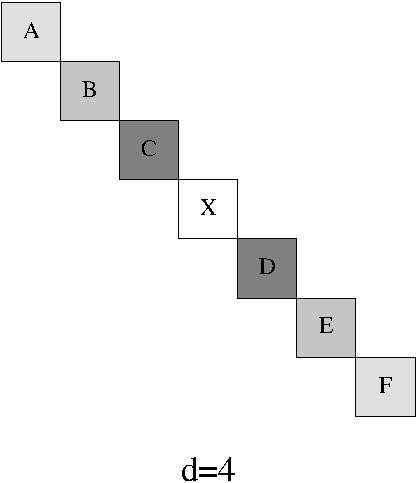
\includegraphics[scale=0.5]{taps4}\hspace{1.5em}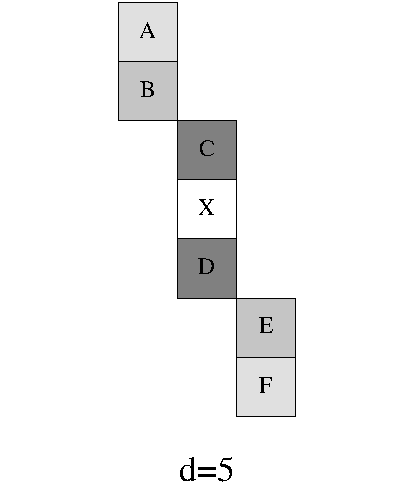
\includegraphics[scale=0.5]{taps5}\hspace{1.5em}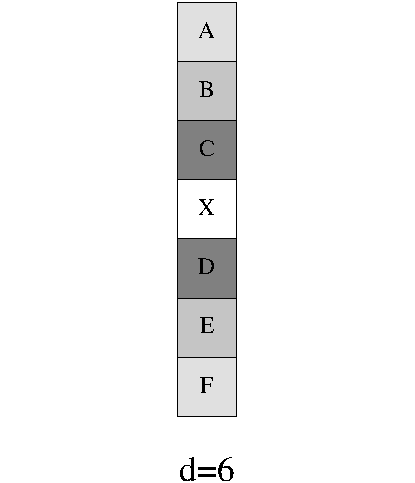
\includegraphics[scale=0.5]{taps6}\hspace{1.5em}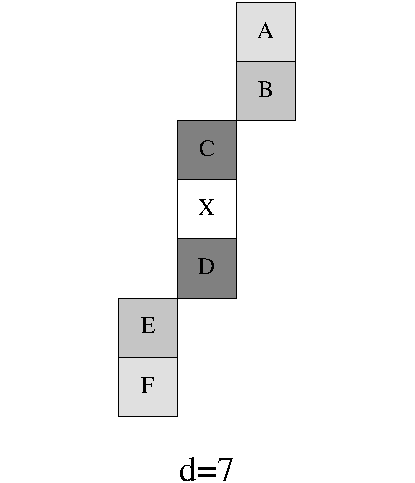
\includegraphics[scale=0.5]{taps7}}

\caption{Position of the directional deringing taps for directions 0 to 7.\label{fig:Position-of-taps}}
\end{figure}


\section{Results}

The deringing filter described here has been implemented in the AV1
codec and can be enabled by configuring the build with the \texttt{-{}-enable-experimental}
and \texttt{-{}-enable-cdef} options.

We tested the deringing filter using the Are We Compressed Yet?~\cite{AWCY}
online testing tool. The results for still images are shown in Table.~\ref{tab:bd-rate}
for the objective-1-fast test set.

\begin{table}
\caption{Deringing filter Bj�ntegaard-delta~\cite{Testing-draft} rate for
still images (lower is better) in Daala.\label{tab:bd-rate}}
\centering{%
\begin{tabular}{cccccc}
\hline 
Bitrate (bpp) & PSNR & CIEDE 2000 & PSNR-HVS & SSIM & MS-SSIM\tabularnewline
\hline 
High-latency & -2.09\% & -1.97\% & -0.74\% & -1.69\% & -0.94\%\tabularnewline
Low-latency & -3.94\% & -3.68\% & -2.38\% & -3.37\% & -2.52\%\tabularnewline
Low-latency, cpu-used=4 & -7.63\% & -7.23\% & -5.20\% & -7.67\% & -5.73\%\tabularnewline
\hline 
\end{tabular}}

\end{table}


\section{Conclusion}

We have demonstrated an effective algorithm for removing ringing artifacts
from coded images and videos. The proposed CDEF algorithm is based
on the conditional replacement filter (CRF) and a constrained low-pass
filter (CLPF) and takes into account the direction of the patterns
it is filtering to reduce the risk of blurring. Objective results
show a bit-rate reduction up to 7.7\% on video sequences. 

\bibliographystyle{IEEEtran}
\bibliography{daala}

\end{document}
